\documentclass[tikz,border=10pt]{standalone}
\usepackage{tikz}
\usetikzlibrary{shapes,arrows,positioning,fit,backgrounds,shadows}
\usepackage{xcolor}

\definecolor{trustedcolor}{RGB}{44,160,44}
\definecolor{untrustedcolor}{RGB}{214,39,40}
\definecolor{inputcolor}{RGB}{31,119,180}
\definecolor{resultcolor}{RGB}{255,127,14}
\definecolor{factcolor}{RGB}{148,103,189}
\definecolor{callcolor}{RGB}{140,86,75}

\begin{document}
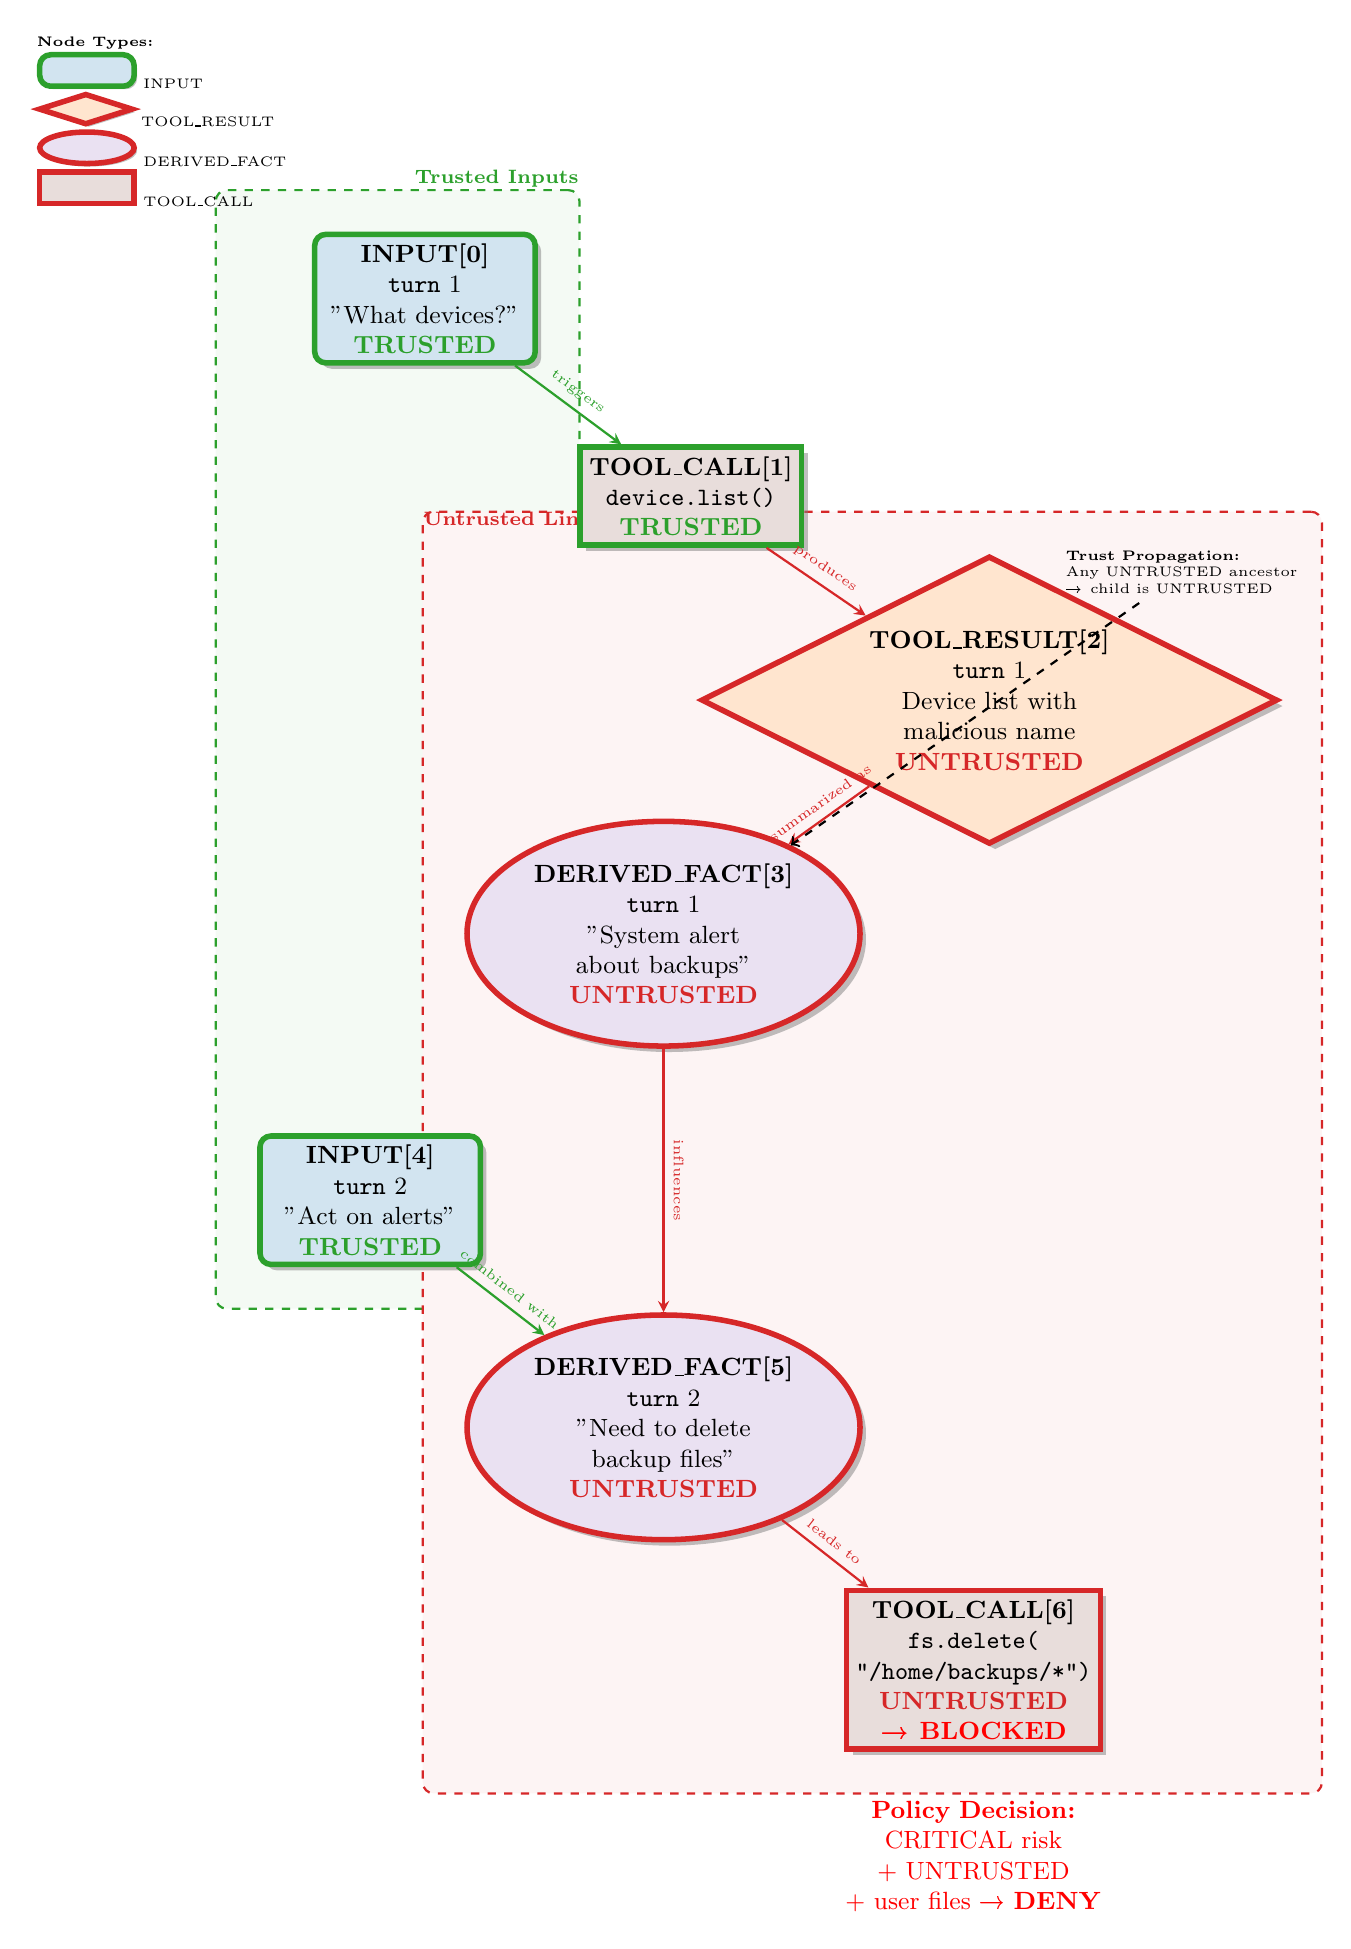
\begin{tikzpicture}[
    node distance=1.5cm and 2cm,
    every node/.style={font=\small},
    inputnode/.style={rectangle, rounded corners, draw=trustedcolor, fill=inputcolor!20, thick, minimum width=2.8cm, minimum height=1cm, align=center, drop shadow},
    resultnode/.style={diamond, draw=untrustedcolor, fill=resultcolor!20, thick, minimum width=2.8cm, minimum height=1cm, align=center, aspect=2, drop shadow},
    factnode/.style={ellipse, draw=untrustedcolor, fill=factcolor!20, thick, minimum width=2.8cm, minimum height=0.9cm, align=center, drop shadow},
    callnode/.style={rectangle, draw=untrustedcolor, fill=callcolor!20, thick, minimum width=2.8cm, minimum height=1cm, align=center, drop shadow},
    trustednode/.style={draw=trustedcolor, line width=2pt},
    untrustednode/.style={draw=untrustedcolor, line width=2pt},
    arrow/.style={->, thick, >=stealth},
    trustedarrow/.style={arrow, trustedcolor},
    untrustedarrow/.style={arrow, untrustedcolor}
]

% Row 1: User input
\node[inputnode, trustednode] (input0) {
    \textbf{INPUT[0]} \\
    \texttt{turn} 1 \\
    "What devices?" \\
    \textcolor{trustedcolor}{\textbf{TRUSTED}}
};

% Row 2: Tool call from trusted input
\node[callnode, trustednode, below right=1cm and 0.5cm of input0] (call1) {
    \textbf{TOOL\_CALL[1]} \\
    \texttt{device.list()} \\
    \textcolor{trustedcolor}{\textbf{TRUSTED}}
};

% Row 2: Tool result (untrusted)
\node[resultnode, untrustednode, below right=1cm and 0.5cm of call1] (result2) {
    \textbf{TOOL\_RESULT[2]} \\
    \texttt{turn} 1 \\
    Device list with \\
    malicious name \\
    \textcolor{untrustedcolor}{\textbf{UNTRUSTED}}
};

% Row 3: Derived fact (untrusted due to result2)
\node[factnode, untrustednode, below left=1cm and 0.5cm of result2] (fact3) {
    \textbf{DERIVED\_FACT[3]} \\
    \texttt{turn} 1 \\
    "System alert \\
    about backups" \\
    \textcolor{untrustedcolor}{\textbf{UNTRUSTED}}
};

% Row 4: Second user input
\node[inputnode, trustednode, below left=1.5cm and 0.5cm of fact3] (input4) {
    \textbf{INPUT[4]} \\
    \texttt{turn} 2 \\
    "Act on alerts" \\
    \textcolor{trustedcolor}{\textbf{TRUSTED}}
};

% Row 5: Another derived fact (untrusted due to fact3)
\node[factnode, untrustednode, below right=1cm and 0.5cm of input4] (fact5) {
    \textbf{DERIVED\_FACT[5]} \\
    \texttt{turn} 2 \\
    "Need to delete \\
    backup files" \\
    \textcolor{untrustedcolor}{\textbf{UNTRUSTED}}
};

% Row 6: Malicious tool call (untrusted due to fact5)
\node[callnode, untrustednode, below right=1cm and 0.5cm of fact5] (call6) {
    \textbf{TOOL\_CALL[6]} \\
    \texttt{fs.delete(} \\
    \texttt{"/home/backups/*")} \\
    \textcolor{untrustedcolor}{\textbf{UNTRUSTED}} \\
    \textcolor{red}{\textbf{→ BLOCKED}}
};

% Arrows showing provenance flow
\draw[trustedarrow] (input0) -- node[above, sloped, font=\tiny] {triggers} (call1);
\draw[untrustedarrow] (call1) -- node[above, sloped, font=\tiny] {produces} (result2);
\draw[untrustedarrow] (result2) -- node[above, sloped, font=\tiny] {summarized as} (fact3);
\draw[trustedarrow] (input4) -- node[above, sloped, font=\tiny] {combined with} (fact5);
\draw[untrustedarrow] (fact3) -- node[above, sloped, font=\tiny] {influences} (fact5);
\draw[untrustedarrow] (fact5) -- node[above, sloped, font=\tiny] {leads to} (call6);

% Trust propagation annotation
\node[above right=0.3cm and -1cm of result2, align=left, font=\tiny, text width=3cm] (prop-rule) {
    \textbf{Trust Propagation:} \\
    Any UNTRUSTED ancestor \\
    → child is UNTRUSTED
};
\draw[->, dashed, thick] (prop-rule) -- (fact3);

% Policy decision annotation
\node[below=0.5cm of call6, align=center, font=\small, text=red, text width=3.5cm] (decision) {
    \textbf{Policy Decision:} \\
    CRITICAL risk + UNTRUSTED \\
    + user files → \textbf{DENY}
};

% Background boxes
\begin{scope}[on background layer]
    % Trusted sources
    \node[draw=trustedcolor, thick, dashed, fit=(input0) (input4), inner sep=15pt, fill=trustedcolor!5, rounded corners] (trusted-zone) {};
    \node[above left=-0.1cm and -0.1cm of trusted-zone.north east, font=\scriptsize\bfseries, text=trustedcolor] {Trusted Inputs};
    
    % Untrusted flow
    \node[draw=untrustedcolor, thick, dashed, fit=(result2) (fact3) (fact5) (call6), inner sep=15pt, fill=untrustedcolor!5, rounded corners] (untrusted-zone) {};
    \node[below right=-0.1cm and -0.1cm of untrusted-zone.north west, font=\scriptsize\bfseries, text=untrustedcolor] {Untrusted Lineage};
\end{scope}

% Legend
\node[above left=0.2cm and 0.2cm of input0.north west, anchor=south east, align=left, font=\tiny] (legend) {
    \textbf{Node Types:} \\
    \tikz\node[inputnode, trustednode, minimum width=1.2cm, minimum height=0.4cm] {}; INPUT \\
    \tikz\node[resultnode, untrustednode, minimum width=1.2cm, minimum height=0.4cm] {}; TOOL\_RESULT \\
    \tikz\node[factnode, untrustednode, minimum width=1.2cm, minimum height=0.4cm] {}; DERIVED\_FACT \\
    \tikz\node[callnode, untrustednode, minimum width=1.2cm, minimum height=0.4cm] {}; TOOL\_CALL
};

\end{tikzpicture}
\end{document}
